 \documentclass[main.tex]{subfiles}
% 线性变换的转置
\begin{document}
由之前的介绍可知,抽象定义的向量和线性变换都不是矩阵,但是在给定基下,它们又都能唯一地表示为矩阵。线性变换的转置,也需要在更一般的角度得到定义,而且需要为这件事引入更多新概念。

我们首先引入线性泛函的概念,以便定义线性变换的转置。

\begin{definition}[线性泛函与对偶空间]\label{def:II.4.4}
    设$\mathcal{V}$是数域$\mathbb{F}$上的向量空间,从$\mathcal{V}$到$\mathbb{F}$的线性变换称为向量空间$\mathcal{V}$上的\emph{线性泛函(linear functional)},$\mathcal{V}$上的所有线性泛函的集合称为向量空间$\mathcal{V}$的\emph{对偶空间(dual space)},记为$\mathcal{V}^*$。
\end{definition}

线性泛函把一个向量对应为同数域上的一个数。由该定义,若映射$f:\mathcal{V}\rightarrow\mathbb{F}$满足$f\left(\alpha\mathbf{a}+\mathbf{b}\right)=\alpha f\left(\mathbf{a}\right)+f\left(\mathbf{b}\right),\forall\mathbf{a},\mathbf{b}\in\mathcal{V},\alpha\in\mathbb{F}$,则$f$是$\mathcal{V}$上的一个线性泛函,且$\mathcal{V}$的对偶空间$\mathcal{V}^*$就是线性变换空间$\mathcal{L}\left(\mathcal{V},\mathbb{F}\right)$,且有$\mathrm{dim}\mathcal{V}^*=\mathrm{dim}\mathcal{V}$。

\begin{example}\label{exp:II.2.11}
    验证:
    \begin{itemize}
        \item 函数$f\left(x,y,z\right)=3x+5y-z,x,y,z\in\mathbb{R}$是3维实坐标空间$\mathbb{R}^3$上的线性泛函。
        \item 函数$f\left(\mathbf{x}\right)=3\left(\mathbf{x}\cdot\mathbf{x}\right),\mathbf{x}\in\mathbb{R}^n$是$n$维实坐标空间$\mathbb{R}^n$上的线性泛函。
        \item 设$\mathbb{F}^{M\times M}$是数域$\mathbb{F}$上的$M\times M$矩阵的集合,矩阵的迹$\mathrm{tr}A=A_{11}+\cdots+A_{MM},A\in\mathbb{F}^{M\times M}$是$\mathbb{F}^{M\times M}$上的线性泛函。
        \item 设$a_1,\cdots,a_n\in\mathbb{F}$,并定义映射$f:\mathbb{F}^n\rightarrow\mathbb{F},f\left(x_1,\cdots,x_n\right)=a_1x_1+\cdots+a_nx_n,\quad\forall\left(x_1,\cdots,x_n\right)\in\mathbb{F}$,验证$f$是$\mathbb{F}^n$上的线性泛函。这事实上既是两个$n\times 1$列向量的“点乘”,又是一个$1\times n$“行向量”与$n\times 1$“列向量”的矩阵乘。
        \item $\mathcal{C}\left[a,b\right]$是区间$\left[a,b\right]$上的所有连续实值函数的集合,可验证它是数域$\mathbb{R}$上的向量空间\cite{周胜林2012线性代数}[\S 7.1 例1.3]。定义$L:\mathcal{C}\left[a,b\right]\rightarrow\mathbb{R},L\left(g\right)=\int_a^bf\left(t\right)\mathrm{d}t,\quad\forall g\in\mathcal{C}\left[a,b\right]$,验证$L$是$\mathcal{C}\left[a,b\right]$上的线性泛函。
    \end{itemize}
\end{example}

从概念上可以说,线性泛函是$\mathcal{V}$上的线性变换,$\mathcal{V}$的对偶空间是$\mathcal{V}$上的线性变换的空间。但我们没有用$\mathcal{L}\left(\mathcal{V},\mathbb{F}\right)$这种记号,而是用$\mathcal{V}^*$,是因为考虑到$\mathrm{dim}\mathcal{V}=\mathrm{dim}\mathcal{V}^*$,$\mathcal{V}$与$\mathcal{V}^*$更像是并列的概念。我们注意到,作为空间$\mathcal{L}\left(\mathcal{V},\mathbb{F}\right)$,维数应该写成$\mathrm{dim}\mathbb{F}\times\mathrm{dim}\mathbb{\mathcal{V}}$。也就是说,设$\mathrm{dim}\mathcal{V}=N$,则给定$\mathcal{V}$的某组有序基,$\mathcal{V}$的向量的坐标是$N\times 1$“列向量”,而$\mathcal{V}^*$中的线性泛函(它们也是向量)在给定$\mathcal{V}^*$的某组有序基下的坐标是$1\times N$“行向量”。那么,我们能不能进一步在$\mathcal{V}$与$\mathcal{V}^*$之间找到更明确的对应关系,看看$\mathcal{V}$中的某一向量的坐标,“转置”成行向量之后,在$\mathcal{V}^*$中找到的是哪一个线性泛函?这一联系当然需要给定$\mathcal{V}$和$\mathcal{V}^*$的基之后才能被确定。下面我们考察$\mathcal{V}$的基与$\mathcal{V}^*$的基的关系,通过一系列定理的证明找到两者之间的唯一对应性。

\begin{theorem}\label{thm:II.2.18}
    设$\mathcal{V}$是数域$\mathbb{F}$上的有限维向量空间,$\left\{\mathbf{a}_i\right\}$是$\mathcal{V}$的一组基,则对每个$i=1,\cdots,n$,有且只有一个$\mathcal{V}$上的线性泛函$f_i$满足$f_i\left(\mathbf{a}_j\right)=\delta_{ij},\quad i,j=1,\cdots,n$,且$\left\{f_i\right\}$线性无关。
\end{theorem}
\begin{proof}
    “有且只有”由引理\ref{lem:II.2.1}易证,略。下面简要证明“线性无关”。

    设$f=\sum_{i=1}^n\gamma_if_i$,则$f\left(\mathbf{a}_j\right)=\sum_{i=1}^n\gamma_if_i\left(\mathbf{a}_j\right)=\sum_{i=1}^n\delta_{ij}=c_j,j=1,\cdots,n$。特别地,$f=0$(这里的$0$是$\mathcal{V}^*$的零向量)$\Leftrightarrow c_j=0\forall j=1,\cdots,n$。
\end{proof}

由于$\mathrm{dim}\mathcal{V}^*=\mathrm{dim}\mathcal{V}=n$,故$n$个$\mathcal{V}^*$中的线性无关向量就是$\mathcal{V}^*$的一组基,因而上面的定理和推论告诉我们,给定向量空间$\mathcal{V}$上的一组有序基,总能在其对偶空间$\mathcal{V}^*$中找到唯一对应的一组有序基,且$\mathcal{V}^*$的基向量作为$\mathcal{V}$上的线性泛函作用于$\mathcal{V}$的基向量等于克劳内克符号。既然$\mathcal{V}$、$\mathcal{V}^*$的上述两种基总是相互唯一对应的,我们就可以将一者定义为另一者的“对偶基”。

\begin{definition}[对偶基]\label{def:II.2.15}
    设$\mathcal{V}$是数域$\mathbb{F}$上的有限维向量空间。给定$\mathcal{V}$的一组基$B=\left\{\mathbf{a}_i\right\}$,$\mathcal{V}$的对偶空间$\mathcal{V}^*$中的(唯一一组)满足$f_i\left(\mathbf{a}_j\right)=\delta_{ij},\quad i,j=1,\cdots,\mathrm{dim}\mathcal{V}$的基$\left\{f_i\right\}$称为$\left\{\mathbf{a}_i\right\}$的\emph{对偶基(dual basis)}。
\end{definition}

由基的概念,$\mathcal{V}^*$中的任一线性泛函$f\in\mathcal{V}^*$都可以用$\mathcal{V}^*$的任一组基$\left\{f_i\right\}$表出,即$f=\sum_{i=1}^nc_if_i,c_i\in\mathbb{F}$。如果已知$\left\{f_i\right\}$是$\mathcal{V}$的一组基$B=\left\{\mathbf{a}_i\right\}$的对偶基,那么通过与定理\ref{thm:II.2.18}的证明过程类似的方法,可知$c_i=f\left(\mathbf{a}_i\right),i=1,\cdots,n$,故$f=\sum_{i=1}^nf\left(\mathbf{a}_i\right)f_i$,即$f$的第$i$个坐标可通过用$f$作用于有序基$B$的第$i$个向量来获得。同时,任一$\mathcal{V}$中的向量$\mathbf{x}\in\mathcal{V}$都可表示为$\mathbf{x}=\sum_{i=1}^n\xi_i\mathbf{a}_i$。若用$B$的对偶基向量一一作用于$\mathbf{x}$,$f_i\left(\mathbf{x}\right)=\sum_{i=1}^n\xi_if_i\left(\mathbf{a}_i\right)=\sum_{i=1}^n\xi_i\delta_{ij}=\xi_i,i=1,\cdots,n$,即得到$\mathbf{x}$在$B$下的相应坐标,故$\mathbf{x}=\sum_{i=1}^nf_i\left(\mathbf{x}\right)\mathbf{a}_i$,即$\mathbf{x}$的第$i$个坐标可通过用$f_i$作用于向量$\mathbf{x}$来获得。简而言之,对偶基其实就是一种“取坐标的函数”;一个向量在给定基下的第$i$个向量,就用这组基的第$i$个对偶基作用于这个向量来得到。

\begin{example}
    设$\mathbb{F}^{n\times 1}$是数域$\mathbb{F}$上的所有$n\times 1 $“列向量”的集合。由例\ref{exp:II.2.6}可知,仅第$i$个分量为1,其余分量均为零的$n$个列向量$E^i$是$\mathbb{F}^{n\times 1}$的一组规范正交集。由于它们正好有$n$个,且由定理\ref{thm:II.2.4}它们线性无关,故它们就$\mathbb{F}^{n\times 1}$的一组规范正交基。    任一$\mathcal{F}^{n\times 1}$中的列向量$\left(a_1,\cdots,a_n\right)$在这组规范正交基下的坐标就恰为$\left(a_1,\cdots,a_n\right)$。

    由例\ref{exp:II.2.11}最后一例的启发,我们发现$E^{i\intercal}$与任一$\mathcal{F}^{n\times 1}$中的列向量进行矩阵乘,可得到该列向量的第$i$个坐标,可见$E^{i\intercal}$是$E^i$的对偶基。诚然,$E^{i\intercal}E^j=\delta_{ij}$。
\end{example}

接下来我们完成定义线性变换的转置的任务。如图\ref{fig:II.2.2}所示,设数域$\mathbb{F}$上的向量空间$\mathcal{V}$上有一个线性变换$\mathbf{T}$。给定任意向量$\mathbf{a}\in\mathcal{V}$,线性变换后的向量是$\mathbf{Ta}$。如果有一个线性泛函$g$把向量$\mathbf{Ta}$对应为一个数,我们想知道,有没有一个线性泛函$f$能直接作用于$\mathbf{a}$得到相同的数?$f$与$g$的关系是什么?线性变换$\mathbf{T}$的转置$\mathbf{T}^\intercal$就是充当这一问题的答案的一种概念。你想问什么样的$f$能满足$f\left(\mathbf{a}\right)=g\left(\mathbf{Ta}\right),\forall\mathbf{a}\in\mathcal{V}$?答案是$f=\mathbf{T}^\intercal g$。用严格语言的定义如下——

\begin{figure}[htbp]
    \centering
    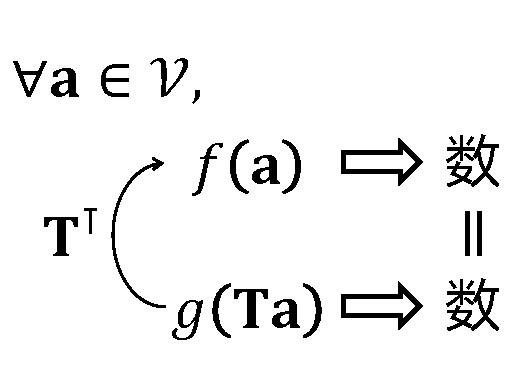
\includegraphics{images/transpose.pdf}
    \caption{线性变换的转置是怎么定义的?设数域$\mathbb{F}$上的向量空间$\mathcal{V}$上有一个线性变换$\mathbf{T}$。给定任意向量$\mathbf{a}\in\mathcal{V}$,线性变换后的向量是$\mathbf{Ta}$。如果有一个线性泛函$g$把向量$\mathbf{Ta}$对应为一个数,我们想知道,有没有一个线性泛函$f$能直接作用于$\mathbf{a}$得到相同的数?$f$与$g$的关系是什么?线性变换$\mathbf{T}$的转置$\mathbf{T}^\intercal$就是充当这一问题的答案的一种概念。你想问什么样的$f$能满足$f\left(\mathbf{a}\right)=g\left(\mathbf{Ta}\right)\forall\mathbf{a}\in\mathcal{V}$?答案是$f=\mathbf{T}^\intercal g$。}
    \label{fig:II.2.2}
\end{figure}

\begin{definition}[线性变换的转置]\label{def:II.2.16}
    设$\mathcal{V},\mathcal{W}$是数域$\mathbb{F}$上的向量空间,$\mathbf{T}:\mathcal{V}\rightarrow\mathcal{W}$是线性变换,对于$\mathcal{W}$上的每一个线性泛函$g\in\mathcal{W}^*$,我们都可以定义一个$\mathcal{V}$上的线性泛函$f\in\mathcal{V}^*$使其满足$f\left(\mathbf{a}\right)=g\left(\mathbf{Ta}\right),\forall \mathbf{a}\in\mathcal{V}$。由$g\in\mathcal{W}^*$到$f\in\mathcal{V}^*$的这一对应规则定义了一个由$\mathcal{W}^*$到$\mathcal{V}^*$的映射$\mathbf{T}^\intercal:\mathcal{W}^*\rightarrow\mathcal{V}^*,\left(\mathbf{T}^\intercal g\right)\left(\cdot\right)=g\left(\mathbf{T}\cdot\right),\forall g\in\mathcal{W}^*$,易验对任一$\mathbf{T}\in\mathcal{L}\left(\mathcal{V},\mathcal{W}\right)$有且只有一个满足上述性质的$\mathbf{T}^\intercal\in\mathcal{L}\left(\mathcal{W}^*,\mathcal{V}^*\right)$,且$\mathbf{T}^\intercal$也是线性变换。我们称$\mathbf{T}^\intercal$为$\mathbf{T}$的\emph{转置(transpose)}。
\end{definition}

以上定义中隐含默认了两件事:1)每个线性变换$\mathbf{T}\in\mathcal{L}\left(\mathcal{V},\mathcal{W}\right)$有且只有一个符合定义的映射$\mathbf{T}^\intercal$;2)$\mathbf{T}^\intercal$也是一个线性变换。1)是比较显然的:假设另有一映射$\mathbf{U}:\mathcal{W}^*\rightarrow\mathcal{V}^*$满足$\left(\mathbf{U}g\right)\mathbf{a}=g\mathbf{Ua}\forall\mathbf{a}\in\mathcal{V}$,则有$\mathbf{U}g=\mathbf{T}^\intercal g\Rightarrow\mathbf{U}\mathbf{T}^\intercal$。关于2),我们可以按照线性变换的定义去验证映射$\mathbf{T}^\intercal$作用于一个线性组合的结果:对任意$g_1,g_2\in\mathcal{W}^*,\gamma\in\mathbb{F}$,由$\left[\mathbf{T}^\intercal\left(\gamma g_1+g_2\right)\right]\left(\mathbf{a}\right)=\left(\gamma g_1+g_2\right)\left(\mathbf{Ta}\right)=\gamma g_1\left(\mathbf{Ta}\right)+g_2\left(\mathbf{Ta}\right)=\gamma\left(\mathbf{T}^\intercal g_1\right)\left(\mathbf{a}\right)+\left(\mathbf{T}^\intercal g_2\right)\left(\mathbf{a}\right)\forall\mathbf{a}\in\mathcal{V}$可知$\mathbf{T}^\intercal\left(\gamma g_1+g_2\right)=\gamma\left(\mathbf{T}^\intercal g_1\right)+\mathbf{T}^\intercal g_2$,故$\mathbf{T}^\intercal$是线性变换。

下面的定理告诉我们,一个线性变换$\mathbf{T}$与其转置$\mathbf{T}^\intercal$在给定基和对偶基下的矩阵之间的关系就是矩阵转置。

\begin{theorem}\label{thm:II.2.19}
    设$\mathcal{V},\mathcal{W}$分别是数域$\mathbb{F}$上的$n,m$维有限维向量空间,给定以下基及其对偶基:$B=\left\{\mathbf{a}_i\right\}\subset\mathcal{V},B^*=\left\{f_i\right\}\subset\mathcal{V}^*,B^\prime=\left\{\mathbf{b}_i\right\}\subset\mathcal{W},B^{\prime *}=\left\{g_i\right\}\subset\mathcal{W}^*$,且令$\mathbf{T}:\mathcal{V}\rightarrow\mathcal{W}$是线性变换,$A$是$\mathbf{T}$在$B,B^\prime$下的坐标矩阵,$B$是$\mathbf{T}^\intercal$在$B^*,B^{\prime *}$下的坐标矩阵,则$B_{ij}=A_{ji},i=1,\cdots,m,j=1,\cdots,n$。
\end{theorem}
\begin{proof}
    根据向量的坐标表达式,可以写出
    \begin{align*}
        \mathbf{Ta}_i            & =\sum_{j=1}^mA_{ji}\mathbf{b}_j,i=1,\cdots,n \\
        \mathbf{T}^\intercal g_i & =\sum_{j=1}^nB_{ji}f_j,i=1,\cdots,m
    \end{align*}
    由线性变换转置的定义和对偶基的定义,
    \begin{align*}
        \left(\mathbf{T}^\intercal g_i\right)\left(\mathbf{a}_j\right) & =g_i\left(\mathbf{Ta}_j\right)                    \\
                                                                       & =g_i\left(\sum_{k=1}^m A_{kj}\mathbf{b}_k\right)  \\
                                                                       & =\sum_{k=1}^m A_{kj} g_i\left(\mathbf{b}_k\right) \\
                                                                       & =\sum_{k=1}^mA_{kj}\delta_{ik}                    \\
                                                                       & =A_{ij},i=1,\cdots,m,j=1,\cdots,n
    \end{align*}
    另一方面,由于$\mathbf{T}^\intercal g_i\in\mathcal{V}^*$,故它可用$B^*$表出,再利用关系$f=\sum_{i=1}^nf\left(\mathbf{a}_i\right)f_i$,有
    \begin{align*}
        \mathbf{T}^\intercal g_i & =\sum_{j=1}^n\left(\mathbf{T}^\intercal g_i\right)\left(\mathbf{a}_j\right) f_j \\
                                 & =\sum_{j=1}^n A_{ij}f_j,i=1,\cdots,m
    \end{align*}
    与之前的结果比较可得$A_{ij}=B_{ji},i=1,\cdots,m,j=1,\cdots,n$。
\end{proof}
\end{document}

